\chapter*{Введение}							% Заголовок
\addcontentsline{toc}{chapter}{Введение}	% Добавляем его в оглавление

\newcommand{\actuality}{{\textbf\actualityTXT}}
\newcommand{\progress}{}
\newcommand{\actualityandprogress}{\textbf{\actualityandprogressTXT}}
\newcommand{\aim}{{\textbf\aimTXT}}
\newcommand{\tasks}{\textbf{\tasksTXT}}
\newcommand{\novelty}{\textbf{\noveltyTXT}}
\newcommand{\influence}{\textbf{\influenceTXT}}
\newcommand{\methods}{\textbf{\methodsTXT}}
\newcommand{\defpositions}{\textbf{\defpositionsTXT}}
\newcommand{\reliability}{\textbf{\reliabilityTXT}}
\newcommand{\probation}{\textbf{\probationTXT}}
\newcommand{\contribution}{\textbf{\contributionTXT}}
\newcommand{\publications}{\textbf{\publicationsTXT}}

{\actualityandprogress}. Методы восстановления измерений в задаче компьютерной томографии можно разделить на интегральные и алгебраические. К интегральным относится метод светки и обратной проекции....

{\aim} ~данной работы являются разработка метода реконструкции, позволяющего учесть присутствие в объекте сильнопоглощающих включений, а так же метода численной интерпретации результатов измерений многокомпонентных объектов.

Для достижения поставленной цели были решены следующие {\tasks}:
\begin{enumerate}
  \item построен асимптотически быстрый алгебраический метод реконструкции, основанный на применении быстрого преобразования Хафа.
  \item доказана сходимость построеного алгебраического метода реконструкции, за счет полученного математического выражения градиента быстрого преобразования Хафа.
  \item построен алгоритм реконструкции для объектов, содержащих сильнопоглощающие включения.
  \item построен алгоритм реконструкции, учитывающий покомпонентное ослабление полихроматического спектра.
\end{enumerate}

{\novelty}
\begin{enumerate}
  \item Впервые для реконструкции томографических измерений было применено быстрое преобразование Хафа.
  \item Впервые получено выражение для производной быстрого преобразования Хафа, а так же алгоритм его эффективного вычисления.
  \item Построен алгоритм реконструкции, учитывающий вклад сильно поглощающих включений с помощью оригинальной модели ограничений-неравенств.
  \item Предложена схема обработки данных полихроматического зондирования, при которой восстанавливаются реальные физические концентрации элементов.
\end{enumerate}

{\influence} ~Результаты, полученные в диссертационной работе, используются для обработки данных лабораторных исследований. Построенные алгоритмы лягут в основу программного обеспечения новых моделей промышленных томографов.

Полученное в работе выражение для градиента быстрого преобразования Хафа имеет общетеоретическое значение и уже применяется в области машинного обучения для обратного распространения ошибки в нейронных сетях глубокого обучения через слой БПХ.

{\methods}
Для решения задач реконструкции томографических измерений используются методы теории условной и безусловной оптимизации: градиентные методы оптимизации, квадратичное программирование, регуляризация.
Для ускорения итерации алгебраического метода используются алгоритмы обработки изображений в виде быстрого преобразования Хафа.


{\defpositions}
\begin{enumerate}
  \item Предложен эффективный вычислительный метод решения задачи томографической реконструкции FHT-SIRT, основанный на алгебраическом подходе, который позволяет снизить асимптотическую оценку сложности вычисления итерации с $O(n^3)$ до $O(n^2~\log n)$, что подтвержается численными экспериментами и замерами времени работы программной реализации алгоритма.
  \item Проведено математическое обоснование сходимости предложенного метода.
  \item Предложен метод реконструкции на основе квадратичного программирования, который позволяет уменьшить артефакты на восстановленном изображении, вызванные наличием сильно поглощающих областей в зондируемом объекте.
  \item Предложен алгебраический метод реконструкции для случая полихроматического зондирования, который решает оптимизационную задачу реконструкции относительно линейной комбинации концентраций с ограничениями-неравенствами на их область значений.
\end{enumerate}


{\reliability} полученных результатов обеспечивается модельными экспериментами и численными симуляциями, а так же экспериментами с восстановлением реально измеренных в лабораторных условиях образцов.\ Результаты находятся в соответствии с результатами, полученными другими авторами.


{\probation}
Основные результаты работы докладывались~на: конферециях 
35-я конференция молодых ученых и специалистов «Информационные технологии и системы» (2012, 19 - 25 августа, Петрозаводск, Россия),
11th Biennal Conference on High Resolution X-Ray Diffraction and Imaging (XTOP 2012, St. Petersburg, Russia), 
29th European Conference on Modelling and Simulation (ECMS 2015, Albena, Bulgaria),
Eighth International Conference on Machine Vision (ICMV 2015, Barcelona, Spain),
на общефизическом семинаре ИПТМ РАН (октябрь 2016).

{\contribution} Все результаты диссертации, вынесенные на защиту, получены автором самостоятельно.
Автором самостоятельно реализованы методы восстановления FHT-SIRT из первой главы, барьерных функций из второй, метод взвешанных невязок из третьей, проведены численные экспериметны по обработке реальных и модельных данных.
Постановка задач и обсуждение результатов проводились совместно с научным руководителем.
Генерация модельных данных для экспериментов в полихроматике проводилась аспирантом факультета КН НИУ ВШЭ Ингачевой А.~С. 
Программная имплементация метода мягких ограничений, использованная для сравнения с методом барьерных функций во второй главе, принадлежит Соколову В.~В.
Измерения для экспериментов по восстановлению зуба со свинцовым включением производились на лабоработном источнике ИК РАН в лаборатории рефлектометрии и малоуглового рассеяния.
Многие аспекты исследований в разное время обсуждались с Чукалиной М.~В., Николаевым Д.~П., Бузмаковым А.~В., Ингачевой А.~С., Соколовым В.~В.


\ifthenelse{\equal{\thebibliosel}{0}}{% Встроенная реализация с загрузкой файла через движок bibtex8
    \publications\ Основные результаты по теме диссертации изложены в 11 печатных изданиях, 
    3 из которых изданы в журналах, рекомендованных ВАК, 
    6 "--- в тезисах докладов.%
}{% Реализация пакетом biblatex через движок biber
%Сделана отдельная секция, чтобы не отображались в списке цитированных материалов
  \begin{refsection}%
    \printbibliography[heading=countauthorvak, env=countauthorvak, keyword=biblioauthorvak, section=1]%
    \printbibliography[heading=countauthornotvak, env=countauthornotvak, keyword=biblioauthornotvak, section=1]%
    \printbibliography[heading=countauthorconf, env=countauthorconf, keyword=biblioauthorconf, section=1]%
    \printbibliography[heading=countauthor, env=countauthor, keyword=biblioauthor, section=1]%

    \publications\ Основные результаты по теме диссертации изложены в \arabic{citeauthor} печатных изданиях \nocite{PruBuzNik13, Prun2013Crys, Vestnik2016, Prun2013AutomAndRemCont, buz_jac_2015, chukalina2014xray}, 
    \arabic{citeauthorvak} из которых изданы в журналах, рекомендованных ВАК %\nocite{PruBuzNik13, Prun2013Crys, Vestnik2016}, 
    \arabic{citeauthorconf} "--- в тезисах докладов \nocite{itas2015Prun,itas2015Ingacheva,ecms2015Chukalina, icmv2015Chukalina, embc2013Buzmakov, nikolaevfast}.
  \end{refsection}
} % Характеристика работы по структуре во введении и в автореферате не отличается (ГОСТ Р 7.0.11, пункты 5.3.1 и 9.2.1), потому её загружаем из одного и того же внешнего файла, предварительно задав форму выделения некоторым параметрам

\textbf{Объем и структура работы.} Диссертация состоит из~введения, четырёх глав, заключения и~двух приложений.
%% на случай ошибок оставляю исходный кусок на месте, закомментированным
%Полный объём диссертации составляет  \ref*{TotPages}~страницу с~\totalfigures{}~рисунками и~\totaltables{}~таблицами. Список литературы содержит \total{citenum}~наименований.
%
Полный объём диссертации составляет
\formbytotal{TotPages}{страниц}{у}{ы}{}, включая
\formbytotal{totalcount@figure}{рисун}{ок}{ка}{ков} и
\formbytotal{totalcount@table}{таблиц}{у}{ы}{}.   Список литературы содержит  
\formbytotal{citenum}{наименован}{ие}{ия}{ий}.



\begin{comment}
Одна из самых важных задач при восстановлении измерений в задаче компьютерной томографии --- избежать появления артефактов.
Ошибки восстановления могут привести к неправильным дальнейшим применениям измеренных объектов
Ошибки возникают на всех этапах формирования томографии, начиная с физических калибровок в аппаратной части и кончая ошибками в визуализации результата.
При разработке ПО для томографа, нужно иметь в виду как возможные причины ошибок, так и специфику задачи, для которой применяется томограф.




\todo{дальше как такового введения нет, идут планы и введения из статей, как наработки для копирования текста.}

1. + что такое томография - позволяет без разрушения восстановить внутреннюю структуру в ppt посмотри о видах томографии	

2. + что такое томограф - это аппаратно-программный комплекс, ты будешь в диссере рассматривать проблемы, возникающие в программной части

3. + из Лешиных тезисов - разные объекты требуют разного при реконструкции - отсюда разное качество реконструкции при использовании разных методов реконструкции
  
4. + но не только методы формируют ошибки результатов восстановления - анализ других источников

5. + описываем самое простое измерение - параллельная схема, монохроматический пучок - здесь первое короткое описание модели формирования сигнала в измерительной схеме

6. приходим к выводу, что алгебраические имеют преимущества над интегральными, поскольку можно учесть и влияние аппаратуры и работать при наличии большого шума
но алгебраические медленные - поэтому надо развивать быстрые реализации, хаф

7. усложним задачу. есть сильнопоглощающие включения - часть ко введению из ecms 2015, icmv 2015 подвести к выводу, что надо создавать и в этом простом для измерения случае (параллельный пучок и монохроматика) принципиально новые методы

8. еще усложним задачу - монохроматику заменим полихроматикой и обретем радости с beam-hardening 2 пути решать - честно или постобработкой измеренных проекций или самой восстановленной картинки.

все это дело объединяем еще раз коротко и выводим актуальность работы.
\end{comment}

\chapter{Современные подходы к решению задачи компьютерной томографии}
\section{Принцип действия томографа}
Опишем основные составные части экспериментальной схемы томографа.
Пример реального экспериментального томографа приведен на рисунке ~\ref{fig:ct_scanner}.

\begin{figure}
\centering
\label{fig:ct_scanner}
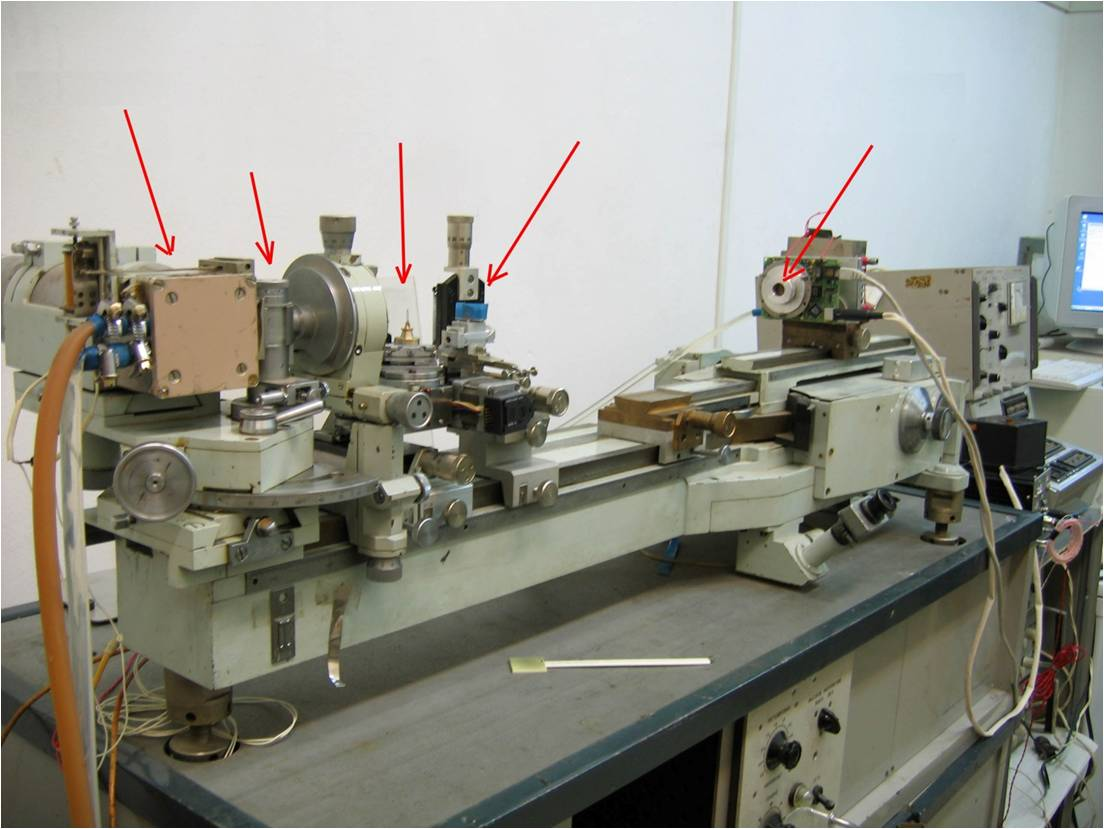
\includegraphics[width=0.7\textwidth]{intro_img/ct_scanner_CIRAS}
\caption{Один из ренгеновских томографов ИК РАН}
\end{figure}

Ренгеновское излучение источника, проходя через предварительные фильтры в виде монохроматора и \textbackslash или коллиматора, попадают на объект исследований.
Объект закреплен на вращающейся относительно источника платформе.
Ренгеновское излучение, проходя через объект, поглощается объектом, в результате чего интенсивность излучения ослабляется в соответствии с законом Бугера-Ламберта-Бера \cite{sivukhin_blb}:

\begin{equation}
\notag
I = I_0 \exp\left( {-\int \! f(l) \mathrm d l }\right),
\end{equation}

где $l$ ---  координата вдоль направления распространения луча, а $f(l)$ --- линейный коэффициент ослабления рентгеновского излучения, $I_0$ --- исходная интенсивность излучения источника, $I$ --- интенсивность излучения, попадающего на измерительный детектор, а интеграл берется вдоль прямой $l$.

Прошедшее через объект излучение регистрируется позиционно-чувствительным детектором.
После дискретизации отклика матрицы детектора даные поступают на обработку ПО реконструкции, которое восстанавливает линейный коэффициент ослабления по набору таких измерений объекта под разными углами проекции.
Для того, чтобы понять принцип работы алгоритмов реконструкции, нужно подробнее описать модель формирования измерений.
Рассмотрим в качестве примера схему эксперимента с параллельным пучком излучения.

\section{Измерения с параллельным пучком}
Несмотря на свою простоту, схема измерений 2D сечения объекта параллельным пучком рентгеновского излучения является ``ядром'' всех алгоритмов восстановления КТ и имеет много применений на практике.
В реальных экспериментальных схемах параллельный пучок рентгеновского излучения можно получить на синхротронах, в лабораторных условиях при использовании монохраматоров, а так же в результате пересчета измерений в веерной 2D геометрии, которая, в свою очередь, возникает в центральном сечении конуского пучка.
Параллельной формой может обладать только пучок монохроматического излучения. 

\begin{figure}[h!]
  \centering
  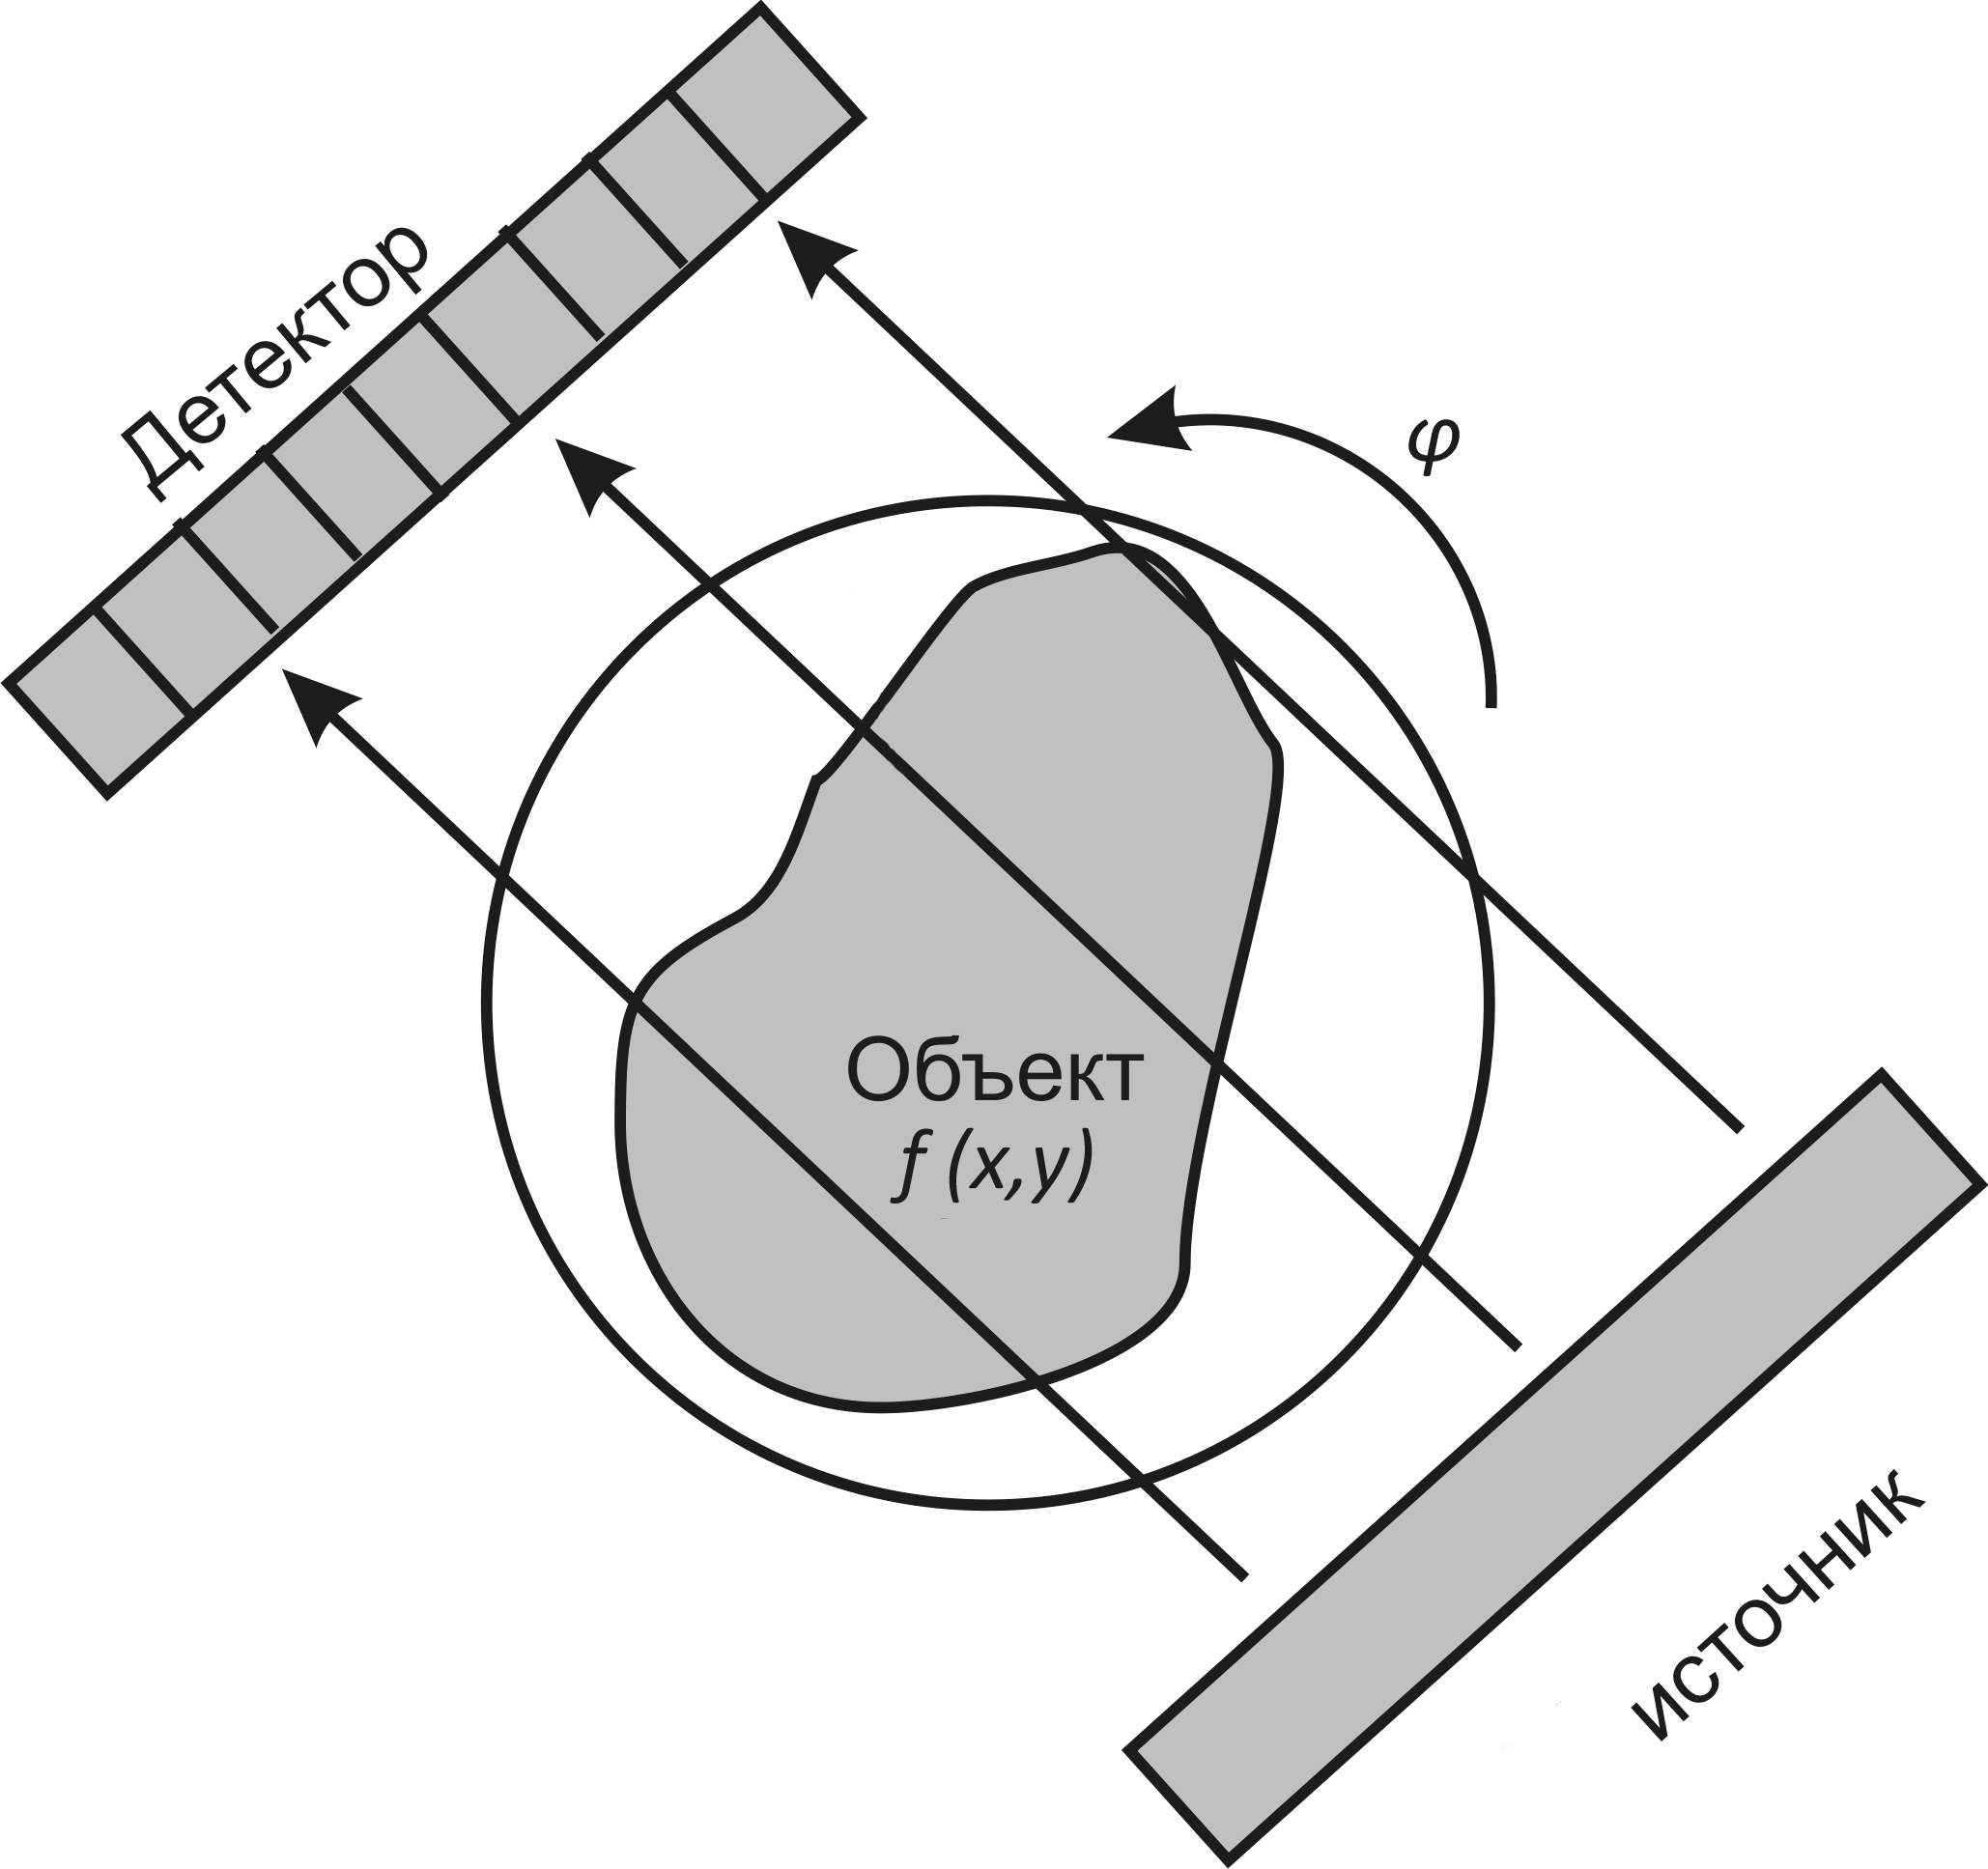
\includegraphics[width=0.5\textwidth]{part1_img/experiment}
  \caption{Схема измерений с параллельным пучком (2D)}
  \label{fig:experiment}
\end{figure}

Схема измерений изображена на рис. ~\ref{fig:experiment}.
Единичного измерения характеризуется двумя параметрами: углом поворота объекта и позицией ячейки детектора, к которой данное измерение относится.
Бесконечно тонкий рентгеновский луч, проходящий под углом $\varphi$  через объект на расстоянии $\xi$  от начала координат, описывается выражением
\begin{equation}\notag
  x\cos\varphi + y\sin\varphi = \xi.
\end{equation}
Тогда регистрируемый в пикселе детектора $\xi$ сигнал имеет интенсивность:
\begin{equation}\notag
  I(\varphi, \xi) = I_0 \exp\left( {-\iint \! \mathrm d x \mathrm d y f(x,y)\delta(x\cos\varphi + y\sin\varphi - \xi)}\right).
\end{equation}
Прологарифмировав обе стороны данного выражения, обозначаем измеренные данные как
\begin{equation}\notag
  p(\varphi, \xi) = \ln \left (\frac{I_0}{I(\varphi, \xi)} \right),
\end{equation}
получим преобразование Радона функции $R[f](\varphi, \xi)$:
\begin{equation}\notag
  p(\varphi, \xi)= \iint \! \mathrm d x \mathrm d y f(x,y)\delta(x\cos\varphi + y\sin\varphi - \xi) = R[f](\varphi, \xi).
\end{equation}
Суть задачи реконструкции в томографии --- восстановление двумерной функции сечения объекта ($f(x,\ y)$) по набору ее линейных интегралов вдоль конечного числа направлений, соответствующих проекционным углам, по набору проекций ($I(\varphi, \xi)$), или обращение преобразования Радона: $\hat{f}(x, y) = R^{-1}[p(\varphi, \xi)](x, y)$.

\section{Методы восстановления}
Задача восстановления изображения характеристики объекта по набору зарегистрированных проекций является задачей обращения преобразования Радона при условии конечного числа направлений проекции.
Существует два основных подхода к восстановлению измерений компьютерной томографии.

Первая группа методов --- интегральные \cite{herman2013mathematical, hsieh2009computed}  --- подходит к решению задачи обращения преобразования Радона аналитически. 
Основной метод восстановления здесь --- метод свертки и обратной проекции (Filtered Backprojection, FBP) \cite{buzug2008computed}.
В основе этого метода лежит использование теоремы о центральном сечении, которая устанавливает связь между одномерным преобразование фурье от преобразования Радона по сдвигам $\hat{R[f](\cdot, \varphi)}$ и двумерным преобразованием фурье исходной функции $\hat{f}(u, v)$.
Для реконструкции искомой функции $f$ применяется явная формула обращения преобразования Радона:
$$
f(x,\ y) = \frac {1} {(2 \pi)^2} \int_0^\pi {
  \left(R[f](\dot,\ \varphi) * h\right)(x \cos \varphi + y \sin \varphi)
} \mathrm d \varphi
$$,
где $h$ это такая одномерная функция, что ее преобразование Фурье $\hat{h}(\omega) = |\omega|$, за $R[f](\dot,\ \varphi) * h$ обозначена свертка элементов преобразования радона для фиксированого угла $\varphi$ с этой функцией.
Именно из-за свертки с фильтром $h$ преобразования Радона метод получил свое название.
Применение FBP является стандартом де-факто в компьютерной томографии.
Вычислительная сложность этого метода определяется сложностью вычисления преобразования фурье изображения, т.е. $O(n^2 \log n)$.
Другой подход к выводу формулы обращения преобразования Радона, а так же анализа необходимого числа измерений, приводится в работах Вайнштейна, Орлова \cite{vainstein_orlov, orlov}.

Интегральный, или аналитический, подход работает с измерениями томографа как с непрерывной функцией, явно решая задачу восстановления.
Данная группа методов является вычислительно эффективной, однако может порождать некачественные востановления, содержащие высокий уровень шума и артефакты \cite{Lucas_sota_ir_survey_2015_radiology}.
Интегральные методы очень чувствительны к наличию шумов в иземенных данных, обоснованная плохой обусловленностью оператора обращения преобразования Радона. 
Так же эти методы требуют наличия большого количества проекционных углов и их равномерного распределения.
Интегральные методы не позволяют учесть априорных знаний о специфике восстанавливаемых объектов.

% дополнить описание FBP формулами

Вторая группа методов --- алгебраические \cite{algebraic_methods}. 
Алгебраические методы решают задачу восстановления распределения линейного коэффициента ослабления рентгеновского излучения в объекте в виде решения СЛАУ.
Уже на этапе моделирования происходит переход к дискретному представлению восстанавливаемой функции, то есть к растровому изображению.
Происходит переход от непрерывных функций $f(x,y), p(\varphi, \xi)$ к дискретным изображениям $f_{ij}, p_{kj}$.
Непрерывное преобразование Радона $R[f](\varphi, \xi)$ для дискретных изображений при конечном наборе углоа проекции принимает вид преобразования Хафа для прямых \cite{Ginkel04ashort}.
Если рассматривать изображения как конечномерные вектора в линейных пространствах размерностей $n \times n$ и $n_\varphi \times n$, то линейному преобразованию Хафа будет соответствовать некоторая матрица $W \in \mathrm{Mat}(\mathbb R, n n \times n_\varphi n)$.
Восстановление сводится к решению СЛАУ большой размерности $Wf = p$.

Первым алгоритмом из семейства алгебраических методов был ART (Algebraic Reconstruction Technique) \cite{GORDON1970471}, в котором авторы применили итерационный метод Качмажа (Kaczmarz) \cite{Kaczmarz1937} решения СЛАУ.
Сам метод Качмажа является частным случаем метода покоординатного спуска или, если речь идет о рандомизированной версии --- стохастического градиенты \cite{needell2014stochastic}.

В зависимости от типа градиентного спуска выделяют разные группы алгебраических методов: SART \cite{sart}, SIRT \cite{GILBERTSIRT}.
В SIRT за один шаг обновления значения переменной используются значения по всем проекционным лучам, в ART --- по одному лучу, в SART --- по всем лучам одного угла проекции.
Введем обозначения: 

\begin{itemize}
	\item $W^{\mathrm T}_j$ --- строка матрицы Хафовской проекции $W$, отвечает за проекцию вдоль выделенной прямой $j$.
	\item $W^\varphi$ --- элемент декомпозиции проекции Хафа по углам. То есть умножение на эту матрицу дает элементы проекции по всем сдвигам но только для угла $\varphi$, а полная матрица $W = \sum W^\varphi$.
	\item $W^{\mathrm T}$ --- транспонированная матрица $W$. Ее умножение на элемент пространства проекций эквивалентен обратному проецированию (backprojection).
	\item $\gamma$ --- параметр релаксации
\end{itemize}

Тогда различия между одним шагом итерации методов ART, SART и SIRT будут выглядеть как это представлено в таблице \ref{tb:art_sart_sirt}:

\begin{table}[h]
\label{tb:art_sart_sirt}
\begin{tabular}{c|c|c}
ART & SART & SIRT \\ \hline
для каждого луча & для каждого угла & для всех лучей\\
$j = 1 \dots N * N_\varphi$ & $\varphi_k$ & \\
$\hat{f} = f - \gamma \mathrm W^{\mathrm T}_j(\mathrm W f - p)$ &
$\hat{f} = f - \gamma \mathrm {W^{\varphi_k}}^{\mathrm T}(\mathrm W f - p)$ &
$\hat{f} = f - \gamma \mathrm W^{\mathrm T}(\mathrm W f - p)$ \\
\end{tabular}
\\
\centering
\caption{Различия в шаге итерации у алгебраических методов}
\end{table}

Варьироваться в методах восстановления могут стратегии релаксации \cite{art_regparam} т.е. поведения $\gamma$ на каждом шаге, и перебора проекций \cite{art_pointschoice}, то есть порядка выбора $\varphi_k,\ j$.
Итеративная природа данных методов позволяет управлять процессом восстановления, используя регуляризацию и априорные знания об объекте исследования.
Так же одним из преимуществ алгебраических методов является довольно общая постановка задачи оптимизации, что позволяет использовать общие наработки теории итеративной градиентной оптимизации для улучшения качества восстановления и скорости сходимости алгоритма.
В последнее время  интерес к итерационной оптимизации особенно сильно возрос в связи с бурным развитием технологий обучения нейронных сетей \cite{battiti1992first, le2011optimization}.
В частности появляются адаптивные методы автоподбора величины шага градиента \cite{kingma2014adam, duchi2011adaptive, zeiler2012adadelta}, добавление затухания направления градиента \cite{qian1999momentum, nesterov1983method}.

Сравнения показывают, что алгебраические методы позволяют достичь лучшего качества восстановления \cite{sirt_less_artifacts, Lucas_sota_ir_survey_2015_radiology}.
В некоторых случаях, использование итерационных методов восстановления позволяет снизить дозу облучения на 70\% \cite{Willemink2013}, что особенно важно при применении томографии в медицине и биологии.
Так же встречаются гибридные методы, в которых итеративное применение интегрального восстановления используется для улучшения качества восстановленных картин.
Хотя концептуально алгебраические методы проще интегральных и лучше справляются с наличием высокого уровня шума в проекциях, они проигрывают последним по времени реконструкции.
Один из способов ускорить восстановление алгебраических методов --- применение распараллеливания на базе графических процессоров \cite{buz2011cuda}.
Другой возможный способ --- применение асимптотически более эффективных алгоритмов проекции (сложность итерации обычных алгебраических подходов $O(n_\varphi n^2)$).
Один из таких алгоритмов --- быстрое преобразование Хафа (БПХ) \cite{Brady1998, brady1992fast, hough}, сложность которого $O(n^2 \log n)$.
Оно основано на использовании особого приближения лучей суммирования, называемого диадическими паттернами.
Форма линии вдоль конкретной суммы получается в результате рекурсивной процедуры по размеру изображения, и отличается от традиционного Брезенхемовского приближения прямой.
Степень отклонения от реальных линий при использовании такого приближения подробно исследуется в работе \cite{ershov2015dyadic}.
Авторам удается теоретически подтвердить эмпирическое наблюдение \cite{Brady1998}, что в худшем случае отклонение диадического паттерна от идеальной линии не превышает $\frac 1 6 \log n$, где $n$ --- линейный размер изображения в пикселях.
Таким образом, при увеличении разрешения сканирования неточность приближения абсолютно тонкого луча в БПХ уменьшается с асимптотикой $O\left(\frac {\log n}{n}\right)$.
Авторы так же исследуют величину девиации трехмерного БПХ от идеальных плоскостей \cite{ershov3DHough}.

\section{Наличие сильнопоглощающих включений}

Одна из известных проблем при востановлении измерений рентгеновской томографии --- возникновение артефактов, вызванных наличием металических (или других сильнопоглощающих) включений в структуре объекта \cite{barrett2004artifacts, boas2012ct, nasirudin2015reduction, park2015computed}.
Наблюдаемые искажения выглядят как темные полосы между металическими включениями со светлым полосатым ореолом окружающих тканей.
Столкнуться с такими артефактами можно, например, при медицинском сканировании пациента с металлическими коронками в зубах или костными протезами.
Наличие таких артефактов может затруднить нахождение или создать несуществующую патологию при медицинском анализе, скрыть или привнести трещины и полости при промышленных исследованиях.
Причины возникновения таких артефактов различны: ``огрубление луча'' (beam hardening), рассеяние, Пуассоновский шум, движение и краевые эффекты \cite{boas2012ct}.
Так же причиной возникновения таких артефактов является низкое соотношение сигнал-шум прошедшего излучения.
Чтобы избежать появления этих артефактов, используются различные методики: аппаратные, например, автоматическое управление модуляцие тока и напряжения на рентгеновской трубке, и программные, например, предобработка данных адаптивными фильтрами \cite{zhang2007reducing}.
Например, в \cite{boas2012ct} используется адаптивное расширение детектирующей ячейки в местах дефицита фотонов.
Еще одна группа методов использует измерения, полученные при зондировании различными энергиями \cite{bamberg2011metal, kuchenbecker2015dual}.

Есть методы, в которых модель формирования синограммы учитывается уже на этапе реконструкции.
Модифицированные алгебраические методы тоже используются для решения проблемы металлических артеыфактов: одни используют аппарат условной оптимизации при постановке задачи \cite{zhang2011metal, sidky2008image}, другие --- модифицируют целевую функцию \cite{meyer2010normalized, kotsenas2015ct}.
Так же для уменьшения артефактов, вызванных металическими включенями используют статистические методы реконструкции \cite{jmuller2006, buzug2008computed}.
В отлчие от методов на основе свертки и обратной проекции, в таких методах есть возможность независимого взвешивания каждого проекционного луча.
Алгоритмы на основе метода максимального правдоподобия, такие как MLEM \cite{buzug2008computed, wang1996iterative} и его модифицированная версия $\lambda$-MLEM \cite{oehler2007statistical}, позволяют улучшить качество восстановленного изображения по сравнению с обычной линейной интерполяцией или предположением о пропущенных данных \cite{amirkhanov2012evaluation}.
Сравнение коммерчески доступных методов подавления артефактов \cite{huang2015evaluation} показывает, что эта проблема не является решенной в прикладных применениях компьютерной томографии, артефакты подавляются не полностью, и это активное поле для исследователей алгоритмов КТ.

\begin{comment}

\todo{введение - обзор из статьи аит2013 и бакалаврского диплома}

 Предлагаются новые версии алгоритмов, основанных на алгебраическом подходе, способных работать с сильно зашумлёнными проекциями. Такое условие сформировано необходимостью сокращать время регистрации проекций. Для некоторых применений уменьшение времени регистрации связано с требованием сокращения дозы облучения, для других --- обусловлено высокой динамикой поведения исследуемого объекта. Также следует отметить, что алгебраические методы реконструкции незаменимы, когда речь идет об экспериментах с малым числом проекционных углов и измерениях в ограниченном телесном угле. Только алгебраические методы применимы для решения задач трансмиссионно-эмиссионной томографии, если ослаблением зондирующего и вторичного излучений пренебречь нельзя.




\end{comment}

\section{Учет полихроматического спектра}
Решение задачи томографической реконструкции в условиях полихроматического сканирования \cite{Herman1979bh} до сегодняшнего дня остается актуальной проблемой, несмотря на большое количество исследований, которые ведутся в разных лабораториях мира.
Основные подходы, применяемые сегодня в методе компьютерной томографии, при работе с полихроматическим излучением --- использование двух различающихся спектров для зондирования \cite{graser2009dual, marin_2014_dual_energy_ct, kuchenbecker2015dual}, использование монохроматоров \cite{tan2012beam}, использование спектрально-чувствительных детекторов \cite{sidky2018three}, и особая обработка данных с томографа. 
В первом случае в 2 раза увеличивается радиационная нагрузка на объект исследования, что нежелательно при исследовании, например, живых объектов.
Во втором сильно уменьшается интенсивность исходного излучения.
Применение фильтров уменьшает поток квантов в единицу времени, что при ограниченном времени измерения снижает величину регистрируемого сигнала и, соответственно, повышает отношение шум/cигнал. 
Так же чтобы корректно провести фильтрацию, необходимо априорное знание об элементном составе образца, а оно не всегда доступно.

Остальные три подхода, это предобработка данных \cite{dewulf2012sense}, создание алгоритмов реконструкции, в которых полихроматичность заложена в математической модели, используемой при обратном проецировании, и постобработка восстановленных изображений. 
Пост процессинг восстановленного изображения \cite{krumm2008reducing} при использовании в ядре реконструкции полихроматической модели, не позволяет получить количественной информации о восстанавливаемом объекте, даже если визуальное представление сильно улучшается (в смысле показателей критериев, созданных для визуального контроля качества изображений).
Данный подход не может быть использован в таких областях применения компьютерной томографии, в которых от результатов КТ ждут количественной информации.
Это требуется в случаях, когда информация КТ не является конечной целью, а применяется при дальнейших расчетах и исследованиях.
Т.е. свойства исследуемых материалов должны быть описаны количественно.

Метод, предложенный в \cite{park2016metal} позволяет разделить металлические включения от биологических тканей в исследуемых образцах, при этом исправив артефакты восстановления, вызванные наличием этих включений.
Авторы пользуются явной формулой для вычисления коррекции на этапе пост-обработки, при этом производя оптимизацию ее гиперпараметров на этапе восстановления.
Одно из важных наблюдений авторов состоит в том, что немонохроматичность слабо проявляется в слабопоглощающих тканях, реальная зависимость от спектра присутствует только в металлических включениях.

Второй подход к решению задачи базируется на том, что модель, используемая при обратном проецировании, учитывает эффект полихроматичности.
При этом используются разные приближения \cite{stenner2010dynamic, van2011iterative}.
В работе \cite{brabant2012novel} детально описана процедура реконструкции, она легко применяется к модельным данным, показывает отличные результаты, однако, в ней опущен шаг перехода от нелинейной системы уравнений, которая описывает процесс формирования томографической проекции в полихроматических условиях, к линейной системе, которая потом решается с учетом полихроматичности.
Результаты предварительных исследований показали, что вопрос перехода от нелинейной системы к линейной не является тривиальным, а требует глубокого исследования и описания случаев, для которых при строго соблюденном перечне условий переход вообще является математически корректным.

Наконец, использование предобработки, т.е. коррекции зарегистрированных проекций перед шагом построения синограммы.
Его сильной стороной является тот факт, что если коррекцию удается провести с учетом поглощательных свойств всех включенных в исследуемый объект компонент, то затем можно применять методы реконструкции, созданные для монохроматического зондирования.
Для эффективной реализации такого способа коррекции необходимо создать базу параметров коррекции для типичных классов исследуемых образцов.
Такая база требует постоянного дополнения и перепроверки, с целью дополнительной калибровки корректирующих кривых.
И тем не менее, поскольку часто время реконструкции является важным параметром при создании программного обеспечения, такой процесс подготовки является приемлемым.